\documentclass[a4paper,10pt]{article}
\usepackage[utf8]{inputenc}
\usepackage[margin=1.5cm, bottom=2cm]{geometry}
\usepackage{fancyhdr}
\usepackage{enumitem}
\usepackage{xcolor}
\usepackage{makeidx}
\usepackage[most]{tcolorbox}
\newtcolorbox{osservazioni}{
  colback=gray!8,    % sfondo grigio chiaro
  colframe=white,      % nessun bordo
  arc=2mm,            % angoli smussati
  boxrule=0pt,        % spessore bordo 0
  fontupper=\footnotesize,
  left=2mm, right=2mm, top=2mm, bottom=2mm,
  before skip=7pt,   % niente spazio prima
  after skip=15pt     % niente spazio dopo
}
\newtcolorbox{osservazioni2}{
  colback=gray!8,    % sfondo grigio chiaro
  colframe=white,      % nessun bordo
  arc=2mm,            % angoli smussati
  boxrule=0pt,        % spessore bordo 0
  fontupper=\small,
  left=5mm, right=5mm, top=3mm, bottom=3mm,
  before skip=0pt,   % niente spazio prima
  after skip=30pt     % niente spazio dopo
}
\pagestyle{fancy}
\usepackage{tikz}
\usetikzlibrary{automata, positioning}
\pagestyle{fancy}

\usepackage{makeidx}

%%%%%%%%%%%%%%%%%%%
\newcommand{\EsercitazioneNum}{03}
\newcommand{\Data}{09/10/2025}
\newcommand{\DocType}{Esercitazione} % o "Eserciziario"
\newcommand{\FullTitle}{\DocType\ \EsercitazioneNum}

\newcommand{\Header}{
\noindent
  \small \textbf{Computabilità, Complessità e Logica - a.a. 2025/26} \hfill \textbf{\FullTitle} \\[0.2cm]
  \scriptsize Matteo Liotta, \texttt{matteo.liotta@studenti.units.it} \hfill \Data \\[0.2cm]
  \noindent\makebox[\linewidth]{\rule{\linewidth}{0.4pt}} \\[0.3cm]}

\newcommand{\NewPageHeader}{
  \vfill
  \noindent\makebox[\linewidth]{\rule{\linewidth}{0.4pt}}
  \newpage
  {\Header}
}
%%%%%%%%%%%%%%%%%%%

% Numero di pagina in basso al centro
\fancyhf{}
\fancyfoot[C] \thepage
\renewcommand{\footrulewidth}{0pt} % niente linea in basso
\renewcommand{\headrulewidth}{0pt} % niente linea in alto

\begin{document}

\footnotesize  % font generale più piccolo
\Header\\[0.7cm]

%%%%%%%%%%%%%%%% FOGLIO 3

%% INDEX
\addcontentsline{toc}{section}{Esercitazione 03: \textit{Operazioni di chiusura per Automi Regolari}} 
%%
\noindent\Large \textbf{Esercitazione \EsercitazioneNum}: \textit{Operazioni di chiusura per Automi Regolari}
\begin{osservazioni}
    \textbf{\textit{Nota}}. Sono indicati in \textcolor{blue}{\textit{blu}} gli esercizi che non saranno trattati durante l'esercitazione, bensì lasciati come strumento aggiuntivo di esercitazione individuale. Resta comunque assoluta disponibilità per la loro risoluzione negli incontri successivi, qualora necessario.
\end{osservazioni}

{\normalsize
\begin{itemize}[label=, leftmargin=0pt]

    \item \underline{\textit{\textbf{Determinizzazione di Automi Regolari ND}}}

    %% INDEX
    \addcontentsline{toc}{subsection}{Esercizio 18.} 
    %%
    \item \textbf{Esercizio 18. (*)}\\ 
    Dato il seguente automa regolare non deterministico definito su $\Sigma=\{a,b\}$, se ne rappresenti graficamente la determinizzazione.
    {
    \small
    \begin{center}
    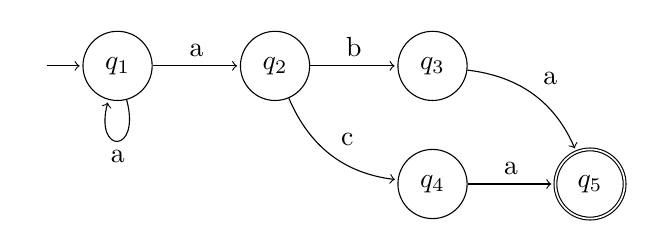
\begin{tikzpicture}[shorten >=1pt, node distance=2cm, on grid, auto]
        \node[state, initial, initial text=] (q1)   {$q_1$};
        \node[state] (q2) [right=of q1] {$q_2$};
        \node[state] (q3) [right=of q2] {$q_3$};
        \node[state] (q4) [below=1.5 of q3] {$q_4$};
        \node[state, accepting] (q5) [right=of q4] {$q_5$};
        
        \path[->]
        (q1) edge [loop below] node {a} (q1)
             edge node {a} (q2)
        (q2) edge node {b} (q3)
             edge [bend right] node {c} (q4)
        (q3) edge [bend left] node {a} (q5)
        (q4) edge node {a} (q5);
    \end{tikzpicture}
    \end{center}
    }%\\[0.1cm]


\begin{osservazioni}
    \underline{\textit{Soluzione.}}
    L'automa, dopo l'operazione di determinizzazione, è il seguente:
    {
    \small
    \begin{center}
    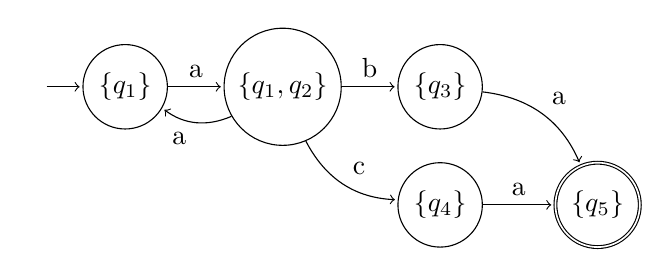
\begin{tikzpicture}[shorten >=1pt, node distance=2cm, on grid, auto]
        \node[state, initial, initial text=] (q1)   {$\{q_1\}$};
        \node[state] (q2) [right=of q1] {$\{q_1,q_2\}$};
        \node[state] (q3) [right=of q2] {$\{q_3\}$};
        \node[state] (q4) [below=1.5 of q3] {$\{q_4\}$};
        \node[state, accepting] (q5) [right=of q4] {$\{q_5\}$};
        
        \path[->]
        (q1)
             edge node {a} (q2)
        (q2) edge [bend left] node {a} (q1)
             edge node {b} (q3)
             edge [bend right] node {c} (q4)
        (q3) edge [bend left] node {a} (q5)
        (q4) edge node {a} (q5);
    \end{tikzpicture}
    \end{center}
    }%\\[0.1cm]
    
    
\end{osservazioni}

    %% INDEX
    \addcontentsline{toc}{subsection}{Esercizio 19.} 
    %%
    \item \textcolor{blue}{\textbf{Esercizio 19. (*)} }\\ 
    Dato il seguente automa regolare non deterministico definito su $\Sigma=\{a\}$, se ne rappresenti graficamente la determinizzazione.
    {
    \small
    \begin{center}
    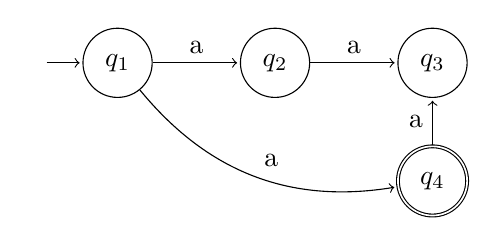
\begin{tikzpicture}[shorten >=1pt, node distance=2cm, on grid, auto]
        \node[state, initial, initial text=] (q1)   {$q_1$};
        \node[state] (q2) [right=of q1] {$q_2$};
        \node[state] (q3) [right=of q2] {$q_3$};
        \node[state, accepting] (q4) [below=1.5 of q3] {$q_4$};
        
        \path[->]
        (q1) edge node {a} (q2)
             edge [bend right] node {a} (q4)
        (q2) edge node {a} (q3)
        (q4) edge node {a} (q3);
        
    \end{tikzpicture}
    \end{center}
    }

\begin{osservazioni}
    \underline{\textit{Soluzione.}}\\
    L'automa, dopo l'operazione di determinizzazione, è il seguente:
    {
    \small
    \begin{center}
    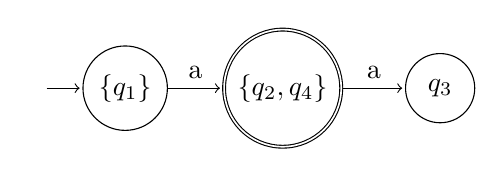
\begin{tikzpicture}[shorten >=1pt, node distance=2cm, on grid, auto]
        \node[state, initial, initial text=] (q1)   {$\{q_1\}$};
        \node[state, accepting] (q2) [right=of q1] {$\{q_2, q_4\}$};
        \node[state] (q3) [right=of q2] {$q_3$};
        
        \path[->]
        (q1) edge node {a} (q2)
        (q2) edge node {a} (q3);
        
    \end{tikzpicture}
    \end{center}
    }
\end{osservazioni}

    \NewPageHeader

    
    %% INDEX
    \addcontentsline{toc}{subsection}{Esercizio 20.} 
    %%
    \item \textbf{Esercizio 20. (**)}\\ 
    Dato il seguente automa regolare non deterministico definito su $\Sigma=\{a,b,c\}$, se ne rappresenti graficamente la determinizzazione.
    {
    \small
    \begin{center}
    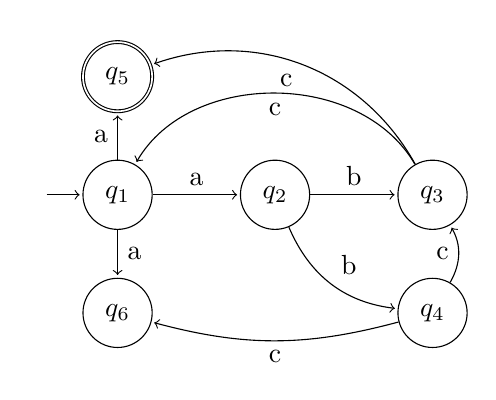
\begin{tikzpicture}[shorten >=1pt, node distance=2cm, on grid, auto]
        \node[state, initial, initial text=] (q1)   {$q_1$};
        \node[state] (q2) [right=of q1] {$q_2$};
        \node[state] (q3) [right=of q2] {$q_3$};
        \node[state] (q4) [below=1.5 of q3] {$q_4$};
        \node[state, accepting] (q5) [above=1.5of q1] {$q_5$};
        \node[state] (q6) [below=1.5of q1] {$q_6$};
        
        \path[->]
        (q1) edge node {a} (q2)
             edge node {a} (q6)
             edge node {a} (q5)
        (q2) edge node {b} (q3)
             edge [bend right] node {b} (q4)
        (q4) edge [bend left=15] node {c} (q6)
             edge [bend right] node {c} (q3)
        (q3) edge [bend right=60] node {c} (q1)
             edge [bend right=40] node {c} (q5);
             
    \end{tikzpicture}
    \end{center}
    }


\begin{osservazioni}
    \underline{\textit{Soluzione.}}\\
    L'automa, dopo l'operazione di determinizzazione, è il seguente:
    {
    \small
    \begin{center}
    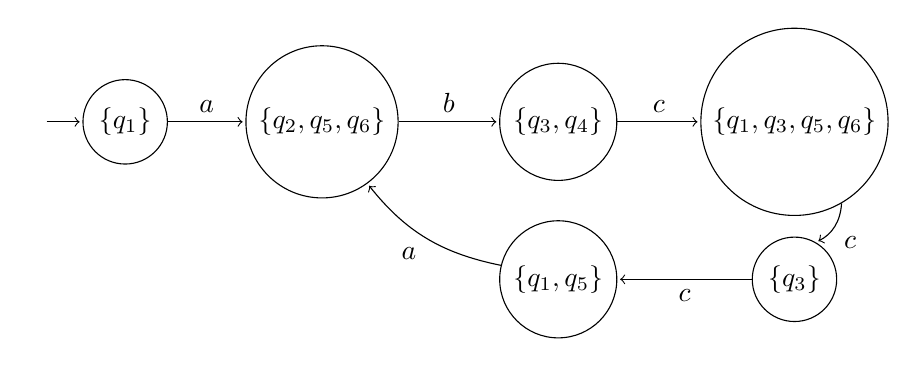
\begin{tikzpicture}[shorten >=1pt, node distance=2cm, on grid, auto]
        \node[state, initial, initial text=] (q1)   {$\{q_1\}$};
        \node[state, right=2.5of q1] (q2)   {$\{q_2, q_5, q_6\}$};
        \node[state, right=3of q2] (q3)   {$\{q_3,q_4\}$};
        \node[state, right=3of q3] (q4)   {$\{q_1,q_3,q_5,q_6\}$};
        \node[state, below=2of q4] (q5)   {$\{q_3\}$};
        \node[state, left=3of q5] (q6)   {$\{q_1,q_5\}$};
        
        \path[->]
        (q1) edge node {$a$} (q2)
        (q2) edge node {$b$} (q3)
        (q3) edge node {$c$} (q4)
        (q4) edge [bend left] node {$c$} (q5)
        (q5) edge node {$c$} (q6)
        (q6) edge [bend left=20] node {$a$} (q2);
        
    \end{tikzpicture}
    \end{center}
    }
\end{osservazioni}


    
    $\\$
    \item \underline{\textit{\textbf{Complementazione di Automi Regolari}}}

    %% INDEX
    \addcontentsline{toc}{subsection}{Esercizio 21.} 
    %%
    \item \textbf{Esercizio 21. (*)}\\ 
    Dato il seguente automa regolare definito su $\Sigma=\{a,b\}$. Si rappresenti graficamente l'automa che accetti il linguaggio regolare complementare:
    
    {
    \small
    \begin{center}
    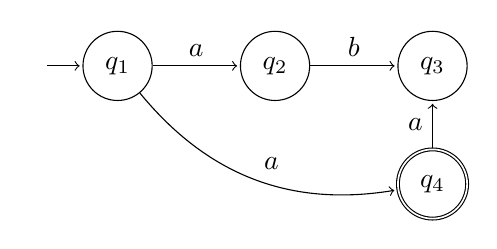
\begin{tikzpicture}[shorten >=1pt, node distance=2cm, on grid, auto]
        \node[state, initial, initial text=] (q1)   {$q_1$};
        \node[state] (q2) [right=of q1] {$q_2$};
        \node[state] (q3) [right=of q2] {$q_3$};
        \node[state, accepting] (q4) [below=1.5 of q3] {$q_4$};
        
        \path[->]
        (q1) edge node {$a$} (q2)
             edge [bend right] node {$a$} (q4)
        (q2) edge node {$b$} (q3)
        (q4) edge node {$a$} (q3);
        
             
    \end{tikzpicture}
    \end{center}
    }

    
\begin{osservazioni}
    \underline{\textit{Soluzione.}}\\
    Ricordiamo come sia necessario completare l'automa degli archi mancanti rispetto alle possibili etichettature in $\Sigma$. Inoltre, ci occupiamo della determinizzazione prima di effettuare la complementazione. Per cui:

    {
    \small
    \begin{center}
    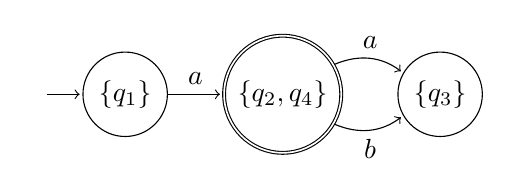
\begin{tikzpicture}[shorten >=1pt, node distance=2cm, on grid, auto]
        \node[state, initial, initial text=] (q1)   {$\{q_1\}$};
        \node[state, accepting] (q2) [right=of q1] {$\{q_2, q_4\}$};
        \node[state] (q3) [right=of q2] {$\{q_3\}$};
        
        \path[->]
        (q1) edge node {$a$} (q2)
        (q2) edge [bend left, above] node {$a$} (q3)
        (q2) edge [bend right, below] node {$b$} (q3);
        
    \end{tikzpicture}
    \end{center}
    }
    è l'automa determinizzato. Eppure, vediamo che al primo e ultimo nodo mancano archi uscenti rispetto ai simboli di $\Sigma$. Essi mappano implicitamente a un nodo di errore da cui impossibile uscire con nessun $\sigma\in \Sigma$.
    
\end{osservazioni}


\NewPageHeader

\begin{osservazioni}
    {
    \small
    \begin{center}
    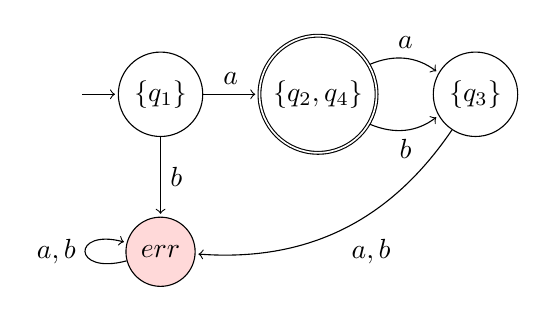
\begin{tikzpicture}[shorten >=1pt, node distance=2cm, on grid, auto]
        \node[state, initial, initial text=] (q1)   {$\{q_1\}$};
        \node[state, accepting] (q2) [right=of q1] {$\{q_2, q_4\}$};
        \node[state] (q3) [right=of q2] {$\{q_3\}$};
        \node[state] (err) [below=of q1, fill=red!15] {$err$};
        
        \path[->]
        (q1) edge node {$a$} (q2)
        (q2) edge [bend left, above] node {$a$} (q3)
        (q2) edge [bend right, below] node {$b$} (q3)
        (q1) edge node {$b$} (err)
        (q3) edge [bend left=30] node {$a,b$} (err)
        (err) edge [loop left] node {$a,b$} (err);
        
    \end{tikzpicture}
    \end{center}
    }
    Da qui è possibile complementare l'automa rispetto ad $F$ e $Q$ ed ottenere:
        {
    \small
    \begin{center}
    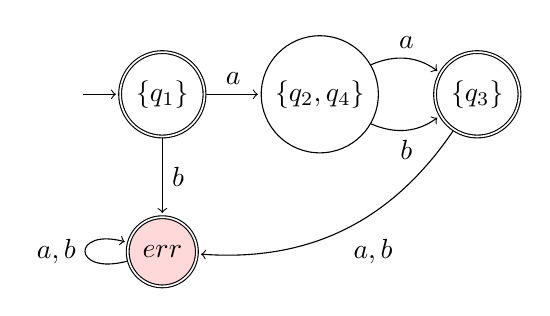
\begin{tikzpicture}[shorten >=1pt, node distance=2cm, on grid, auto]
        \node[state, initial,accepting, initial text=] (q1)   {$\{q_1\}$};
        \node[state] (q2) [right=of q1] {$\{q_2, q_4\}$};
        \node[state, accepting] (q3) [right=of q2] {$\{q_3\}$};
        \node[state, accepting, fill=red!15] (err) [below=of q1] {$err$};
        
        \path[->]
        (q1) edge node {$a$} (q2)
        (q2) edge [bend left, above] node {$a$} (q3)
        (q2) edge [bend right, below] node {$b$} (q3)
        (q1) edge node {$b$} (err)
        (q3) edge [bend left=30] node {$a,b$} (err)
        (err) edge [loop left] node {$a,b$} (err);
        
    \end{tikzpicture}
    \end{center}
    }
\end{osservazioni}
    

    %% INDEX
    \addcontentsline{toc}{subsection}{Esercizio 22.} 
    %%
    \item \textbf{Esercizio 22. (***)}\\ 
    Dato il seguente automa regolare definito su $\Sigma=\{a,b\}$. Si rappresenti graficamente l'automa che accetti il linguaggio regolare complementare.
    {
    \small
    \begin{center}
    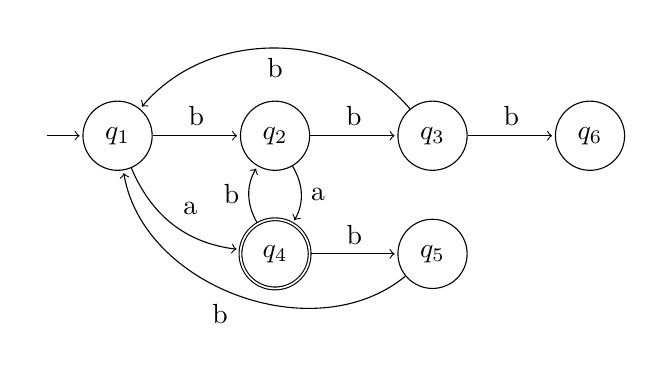
\begin{tikzpicture}[shorten >=1pt, node distance=2cm, on grid, auto]
        \node[state, initial, initial text=] (q1)   {$q_1$};
        \node[state] (q2) [right=of q1] {$q_2$};
        \node[state] (q3) [right=of q2] {$q_3$};
        \node[state, accepting] (q4) [below=1.5 of q2] {$q_4$};
        \node[state] (q5) [below=1.5 of q3] {$q_5$};
        \node[state] (q6) [right=of q3] {$q_6$};

        \path[->]
        (q1) edge node {b} (q2)
             edge [bend right] node {a} (q4)
        (q2) edge node {b} (q3)
             edge [bend left] node {a} (q4)
        (q3) edge node {b} (q6)
             edge [bend right=50] node {b} (q1)
        (q4) edge [bend left] node {b} (q2)
             edge node {b} (q5)
        (q5) edge [bend left=60] node {b} (q1);
        
             
    \end{tikzpicture}
    \end{center}
    }

    \begin{osservazioni}
        \underline{\textit{Soluzione.}}\\
        Seguendo la procedura dell'esercizio precedente, si ottiene il seguente automa, che riconosce il linguaggio complementare.
        {
    \small
    \begin{center}
    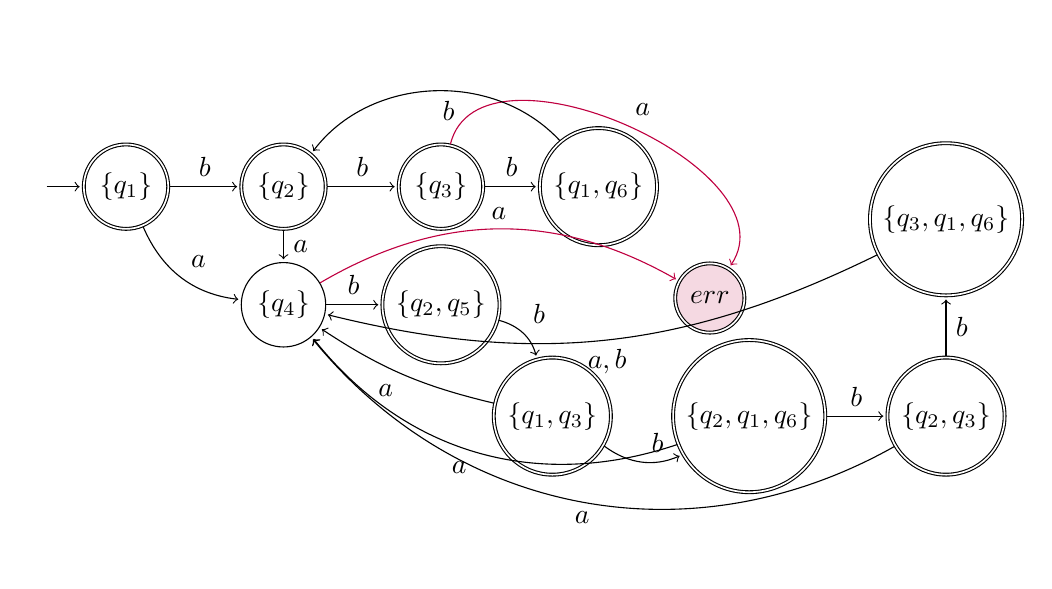
\begin{tikzpicture}[shorten >=1pt, node distance=2cm, on grid, auto]
        \node[state, accepting, initial, initial text=] (q1)   {$\{q_1\}$};
        \node[state, accepting] (q2) [right=of q1] {$\{q_2\}$};
        \node[state, accepting] (q3) [right=of q2] {$\{q_3\}$};
        \node[state] (q4) [below=1.5 of q2] {$\{q_4\}$};
        \node[state, accepting] (q5) [below=1.5 of q3] {$\{q_2,q_5\}$};
        \node[state, accepting] (q6) [right=of q3] {$\{q_1,q_6\}$};
        \node[state, accepting] (q7) [below right=of q5] {$\{q_1,q_3\}$};
        \node[state, accepting] (q8) [right=2.5of q7] {$\{q_2,q_1,q_6\}$};
        \node[state, accepting] (q9) [right=2.5of q8] {$\{q_2, q_3\}$};
        \node[state, accepting] (q10) [above=2.5of q9] {$\{q_3, q_1, q_6\}$};


        %\node[state, accepting] (q8) [right=2.5of q8] {$\{\}$};
        \node[state, accepting] (err) [below right=of q6, fill=purple!15] {$err$};

        \path[->]
        (q1) edge node {$b$} (q2)
             edge [bend right] node {$a$} (q4)
        (q2) edge node {$b$} (q3)
             edge node {$a$} (q4)
        (q3) edge node {$b$} (q6)
             edge [bend left=100, draw=purple] node {$a$} (err)
        (q6) edge [bend right=50] node {$b$} (q2)
        (q4) edge node {$b$} (q5)
             edge [bend left, draw=purple] node {$a$} (err)
        (q5) edge [bend left] node {$b$} (q7)
        (q7) edge [bend right] node {$b$} (q8)
             edge [bend left=10] node {$a$} (q4)
        (q8) %edge [bend right, above] node {$b$} (q7)
             edge [bend left=35] node {$a$} (q4)
             edge  node {$b$} (q9)
        (q9) edge [bend left=40, below] node {$a$} (q4)
             edge [right] node {$b$} (q10)
        (q10) edge [bend left=20, below] node {$a,b$} (q4);
        
    \end{tikzpicture}
    \end{center}
    }
    \end{osservazioni}


\NewPageHeader


    %% INDEX
    \addcontentsline{toc}{subsection}{Esercizio 23.} 
    %%
    \item \textcolor{blue}{\textbf{Esercizio 23. (*) }\\ }
    Dato il seguente automa regolare definito su $\Sigma=\{a,b,c\}$. Si rappresenti graficamente l'automa che accetti il linguaggio regolare complementare.
    {
    \small
    \begin{center}
    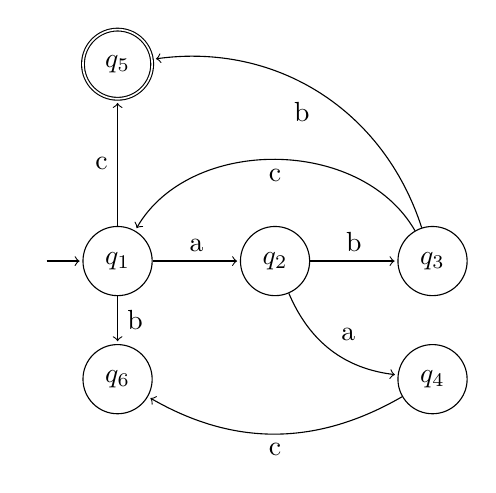
\begin{tikzpicture}[shorten >=1pt, node distance=2cm, on grid, auto]
        \node[state, initial, initial text=] (q1)   {$q_1$};
        \node[state] (q2) [right=of q1] {$q_2$};
        \node[state] (q3) [right=of q2] {$q_3$};
        \node[state] (q4) [below=1.5 of q3] {$q_4$};
        \node[state, accepting] (q5) [above=2.5of q1] {$q_5$};
        \node[state] (q6) [below=1.5of q1] {$q_6$};
        
        \path[->]
        (q1) edge node {a} (q2)
             edge node {b} (q6)
             edge node {c} (q5)
        (q2) edge node {b} (q3)
             edge [bend right] node {a} (q4)
        (q4) edge [bend left] node {c} (q6)
        (q3) edge [bend right=60] node {c} (q1)
             edge [bend right=40] node {b} (q5);
 
    \end{tikzpicture}
    \end{center}
    }

    \begin{osservazioni}
        \underline{\textit{Soluzione.}}\\
        Seguendo la procedura dell'esercizio precedente, si ottiene il seguente automa, che riconosce il linguaggio complementare.
        {
    \small
    \begin{center}
    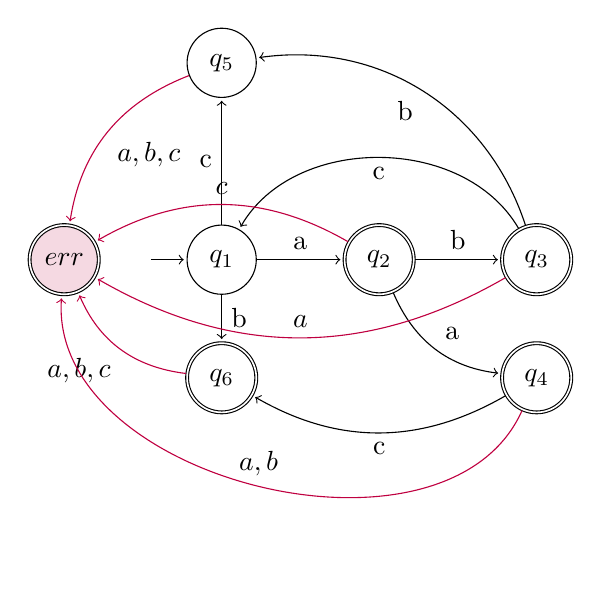
\begin{tikzpicture}[shorten >=1pt, node distance=2cm, on grid, auto]
        \node[state, initial, initial text=] (q1)   {$q_1$};
        \node[state, accepting] (q2) [right=of q1] {$q_2$};
        \node[state, accepting] (q3) [right=of q2] {$q_3$};
        \node[state, accepting] (q4) [below=1.5 of q3] {$q_4$};
        \node[state] (q5) [above=2.5of q1] {$q_5$};
        \node[state, accepting] (q6) [below=1.5of q1] {$q_6$};
        \node[state, accepting, fill=purple!15] (err) [left=2of q1] {$err$};
        
        \path[->]
        (q1) edge node {a} (q2)
             edge node {b} (q6)
             edge node {c} (q5)
        (q2) edge node {b} (q3)
             edge [bend right] node {a} (q4)
        (q4) edge [bend left] node {c} (q6)
        (q3) edge [bend right=60] node {c} (q1)
             edge [bend right=40] node {b} (q5)
        
        (q6) edge [bend left, draw=purple] node {$a,b,c$} (err)
        (q5) edge [bend right,draw=purple] node {$a,b,c$} (err)
        (q2) edge [bend right=30,above, draw=purple] node {$c$} (err)
        (q3) edge [bend left=30,above, draw=purple] node {$a$} (err)
        (q4) edge [bend left=80,above, draw=purple] node {$a,b$} (err);
 
    \end{tikzpicture}
    \end{center}
    }
    \end{osservazioni}

    %% INDEX
    \addcontentsline{toc}{subsection}{Esercizio 24.} 
    %%
    \item \textbf{Esercizio 24. (***)}\\ 
    Sia $L$ linguaggio regolare su $\Sigma =\{a,b\}$, tale per cui
    {\begin{center}
        $L = \{ w \in \Sigma^* \mid w\ \text{ha\ un\ numero\ pari\ di\ a\ e\ multiplo\ di\ 3\ di\ b}\}$
    \end{center}} 
    Si rappresenti graficamente l'automa l'automa che riconosca il linguaggio ad esso complementare.
    $\\\\$
    

    \item \underline{\textit{\textbf{Unione di Automi Regolari}}}


    %% INDEX
    \addcontentsline{toc}{subsection}{Esercizio 25.} 
    %%
    \item \textbf{Esercizio 25. (**)}\\ 
    Siano $L_1, L_2$ linguaggi regolare su $\Sigma =\{a,b\}$, tali per cui
    \begin{itemize}
        \item  $L_1 = \{ w \in \Sigma^* \mid w\ \text{ha\ un\ numero\ pari\ di\ a}\}$
        \item  $L_2 = \{ w \in \Sigma^* \mid w\ \text{ha\ un\ numero\ multiplo di 3\ di\ b}\}$ 
    \end{itemize}
    Si rappresentino graficamente gli automi che riconoscono il linguaggio $L_1,L_2$ e da essi si ricavi l'automa unione, preservando il determinismo.


\NewPageHeader


    \begin{osservazioni}
        \underline{\textit{Soluzione.}}\\
        Si considerano dapprima i due automi regolari indicati, rispettivamente:
        \begin{itemize}
            \item $Aut(L_1)$

{
    \small
    \begin{center}
    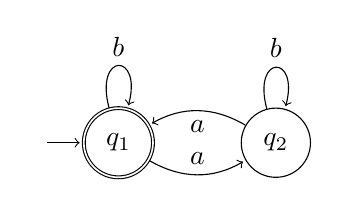
\begin{tikzpicture}[shorten >=1pt, node distance=2cm, on grid, auto]
        \node[state, initial, initial text=, accepting] (q1)   {$q_1$};
        \node[state] (q2) [right=of q1] {$q_2$};
        
        \path[->]
        (q1) edge [loop above] node {$b$} (q1)
        (q1) edge [bend right] node {$a$} (q2)
        (q2) edge [loop above] node {$b$} (q2)
        (q2) edge [bend right] node {$a$} (q1);
        
        
        
         
    \end{tikzpicture}
    \end{center}
    }
    
            
            \item $Aut(L_2)$

{
    \small
    \begin{center}
    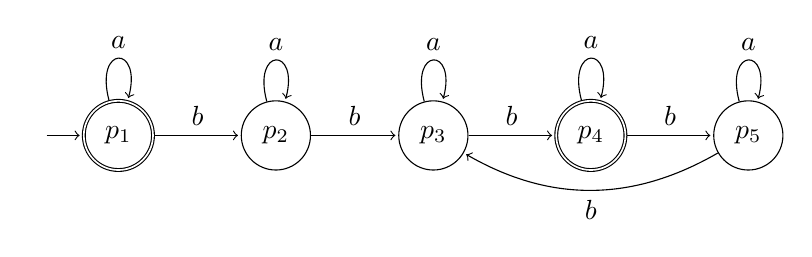
\begin{tikzpicture}[shorten >=1pt, node distance=2cm, on grid, auto]
        \node[state, initial, initial text=, accepting] (p1)   {$p_1$};
        \node[state] (p2) [right=of p1] {$p_2$};
        \node[state] (p3) [right=of p2] {$p_3$};
        \node[state, accepting] (p4) [right=of p3] {$p_4$};
        \node[state] (p5) [right=of p4] {$p_5$};
        
        \path[->]
        (p1) edge [loop above] node {$a$} (p1)
        (p2) edge [loop above] node {$a$} (p2)
        (p3) edge [loop above] node {$a$} (p3)
        (p4) edge [loop above] node {$a$} (p4)
        (p5) edge [loop above] node {$a$} (p5)

        (p1) edge node {$b$} (p2)
        (p2) edge node {$b$} (p3)
        (p3) edge node {$b$} (p4)
        (p4) edge node {$b$} (p5)

        (p5) edge [bend left=30] node {$b$} (p3);
         
    \end{tikzpicture}
    \end{center}
    }
    
    \end{itemize}
    Allora, l'automa unione è il seguente, ottenuto con le coppie di stati raggiungi dalle rispettive funzioni di transizioni $\delta_1$ e $\delta_2$:

    {
    \small
    \begin{center}
    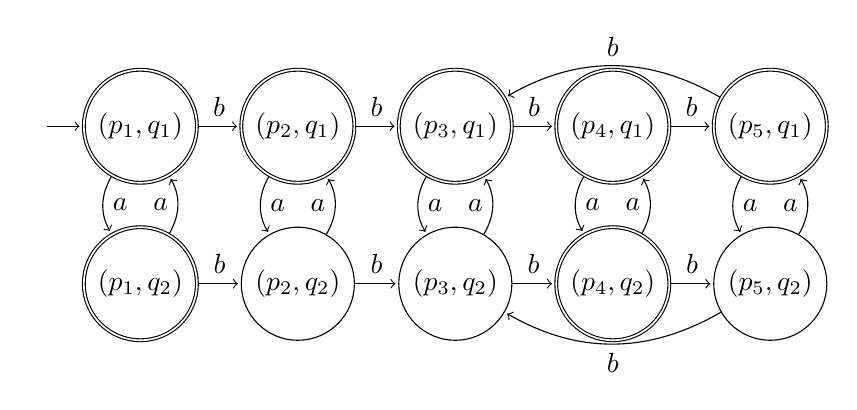
\begin{tikzpicture}[shorten >=1pt, node distance=2cm, on grid, auto]
        \node[state, initial, initial text=, accepting] (p1)   {$(p_1,q_1)$};
        \node[state, accepting] (p2) [right=of p1] {$(p_2,q_1)$};
        \node[state, accepting] (p3) [right=of p2] {$(p_3,q_1)$};
        \node[state, accepting] (p4) [right=of p3] {$(p_4,q_1)$};
        \node[state, accepting] (p5) [right=of p4] {$(p_5,q_1)$};

        \node[state, initial text=, accepting, below=of p1] (q1)   {$(p_1,q_2)$};
        \node[state] (q2) [right=of q1] {$(p_2,q_2)$};
        \node[state] (q3) [right=of q2] {$(p_3,q_2)$};
        \node[state, accepting] (q4) [right=of q3] {$(p_4,q_2)$};
        \node[state] (q5) [right=of q4] {$(p_5,q_2)$};
        
        \path[->]
        (p1) edge [bend right] node {$a$} (q1)
        (p2) edge [bend right] node {$a$} (q2)
        (p3) edge [bend right] node {$a$} (q3)
        (p4) edge [bend right] node {$a$} (q4)
        (p5) edge [bend right] node {$a$} (q5)

        (p1) edge node {$b$} (p2)
        (p2) edge node {$b$} (p3)
        (p3) edge node {$b$} (p4)
        (p4) edge node {$b$} (p5)

        (p5) edge [bend right=30, above] node {$b$} (p3)
        
        (q1) edge [bend right] node {$a$} (p1)
        (q2) edge [bend right] node {$a$} (p2)
        (q3) edge [bend right] node {$a$} (p3)
        (q4) edge [bend right] node {$a$} (p4)
        (q5) edge [bend right] node {$a$} (p5)

        (q1) edge node {$b$} (q2)
        (q2) edge node {$b$} (q3)
        (q3) edge node {$b$} (q4)
        (q4) edge node {$b$} (q5)

        (q5) edge [bend left=30] node {$b$} (q3);
         
    \end{tikzpicture}
    \end{center}
    }
    
    \end{osservazioni}


    %% INDEX
    \addcontentsline{toc}{subsection}{Esercizio 26.} 
    %%
    \item \textcolor{blue}{\textbf{Esercizio 26. (**)}}\\ 
    Sia $L$ linguaggio regolare su $\Sigma =\{a,b\}$, tale per cui
    {\begin{center}
    $L = \{ w \in \Sigma^* \mid w = a^nb^2, n\geq 0\}$\\
    \end{center}}
    Si rappresentino graficamente gli automi che riconoscono il linguaggio $L$ ed $\overline{L}$ e da essi si ricavi l'automa unione; si mostri per tale automa l'accettazione di $\Sigma^*$.

    $\\$
    \item \underline{\textit{\textbf{Intersezione di Automi Regolari}}}


        %% INDEX
    \addcontentsline{toc}{subsection}{Esercizio 27.} 
    %%
    \item \textbf{Esercizio 27. (*)}\\ 
    Si conisderino nuovamente (cfr. es. 9) $L, \overline{L}$, linguaggi regolari su $\Sigma =\{a,b\}$, tali per cui
    {\begin{center}
    $L = \{ w \in \Sigma^* \mid w = a^nb^2, n\geq 0\}$\\
    \end{center}}
    Si rappresenti allora graficamente l'automa prodotto tale da riconoscere l'intersezione dei linguaggi. Quale linguaggio è dunque riconosciuto da tale automa?


\NewPageHeader

    %% INDEX
    \addcontentsline{toc}{subsection}{Esercizio 28.} 
    %%
\item {\textbf{Esercizio 28. (***)}\\ 
    Dati i due automi dei precedenti esercizi, definiti rispettivamente sui linguaggi $\Sigma_1$ e $\Sigma_2$:
    {
    \small
    \begin{center}
    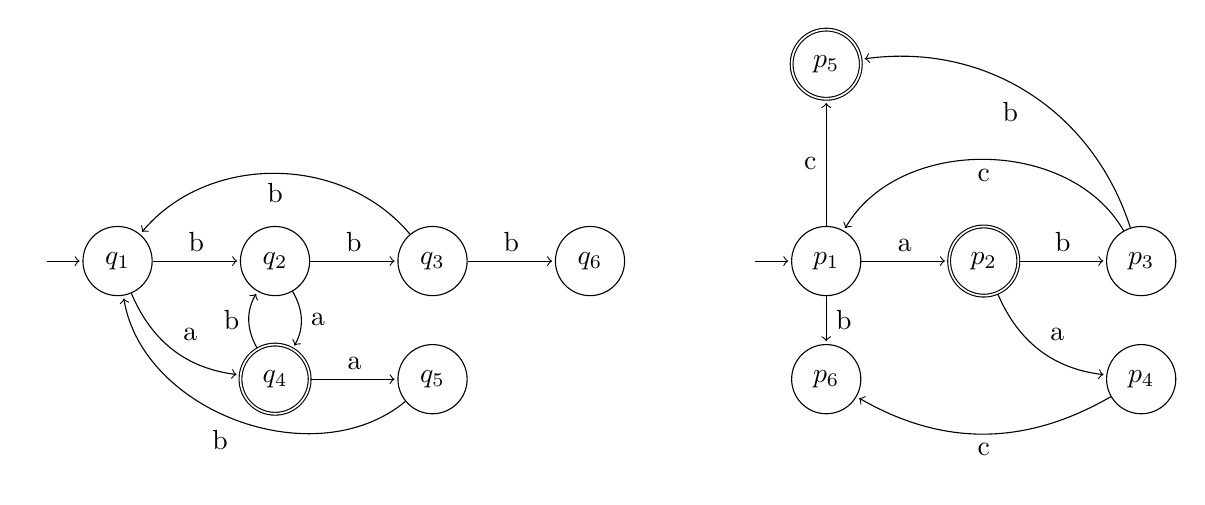
\begin{tikzpicture}[shorten >=1pt, node distance=2cm, on grid, auto]
        \node[state, initial, initial text=] (q1)   {$q_1$};
        \node[state] (q2) [right=of q1] {$q_2$};
        \node[state] (q3) [right=of q2] {$q_3$};
        \node[state, accepting] (q4) [below=1.5 of q2] {$q_4$};
        \node[state] (q5) [below=1.5 of q3] {$q_5$};
        \node[state] (q6) [right=of q3] {$q_6$};

        \path[->]
        (q1) edge node {b} (q2)
             edge [bend right] node {a} (q4)
        (q2) edge node {b} (q3)
             edge [bend left] node {a} (q4)
        (q3) edge node {b} (q6)
             edge [bend right=50] node {b} (q1)
        (q4) edge [bend left] node {b} (q2)
             edge node {a} (q5)
        (q5) edge [bend left=60] node {b} (q1);

        \node[state, initial, initial text=, right=3of q6] (p1)   {$p_1$};
        \node[state, accepting] (p2) [right=of p1] {$p_2$};
        \node[state] (p3) [right=of p2] {$p_3$};
        \node[state] (p4) [below=1.5 of p3] {$p_4$};
        \node[state, accepting] (p5) [above=2.5of p1] {$p_5$};
        \node[state] (p6) [below=1.5of p1] {$p_6$};
        
        \path[->]
        (p1) edge node {a} (p2)
             edge node {b} (p6)
             edge node {c} (p5)
        (p2) edge node {b} (p3)
             edge [bend right] node {a} (p4)
        (p4) edge [bend left] node {c} (p6)
        (p3) edge [bend right=60] node {c} (p1)
             edge [bend right=40] node {b} (p5);
 
    \end{tikzpicture}
    \end{center}
    }
    Si rappresenti graficamente l'automa prodotto, tale da accettare l'intersezione dei linguaggi riconosciuti rispettivamente da ciascun automa.

    \begin{osservazioni}
        \underline{\textit{Soluzione.}}
        L'automa che riconosce il linguaggio intersezione $L_1\cup L_2$ è il seguente:
        {
    \small
    \begin{center}
    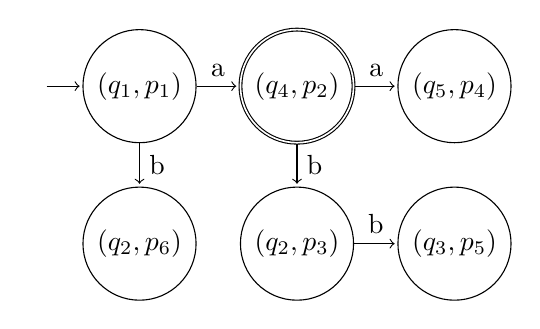
\begin{tikzpicture}[shorten >=1pt, node distance=2cm, on grid, auto]
        \node[state, initial, initial text=] (q1)   {$(q_1,p_1)$};
        \node[state, accepting] (q2) [right=of q1] {$(q_4, p_2)$};
        \node[state] (q3) [right=of q2] {$(q_5, p_4)$};
        \node[state] (q4) [below=of q1] {$(q_2, p_6)$};
        \node[state] (q5) [right=of q4] {$(q_2, p_3)$};
        \node[state] (q6) [right=of q5] {$(q_3, p_5)$};

        \path[->]
        (q1) edge node {a} (q2)
        (q2) edge node {a} (q3)
        (q1) edge node {b} (q4)
        (q2) edge node {b} (q5)
        (q5) edge node {b} (q6);

 
    \end{tikzpicture}
    \end{center}
    }
    \end{osservazioni}

    %% INDEX
    \addcontentsline{toc}{subsection}{Esercizio 29.} 
    %%
    \textcolor{blue}{\item \textbf{Esercizio 29. (*)} \\ }
    Si considerino nuovamente (cfr. es. 9) $L, \overline{L}$, linguaggi regolari su $\Sigma =\{a,b\}$, tali per cui
    {
    \begin{center}
    $L = \{ w \in \Sigma^* \mid w = a^nb^2, n\geq 0\}$\\
    \end{center}
    }
    Si rappresenti allora graficamente l'automa prodotto tale da riconoscere l'intersezione dei linguaggi. Quale linguaggio è dunque riconosciuto da tale automa?

}
\end{itemize}
}
\vfill
\noindent\makebox[\linewidth]{\rule{\linewidth}{0.1pt}}
\end{document}
